 \documentclass[12pt, twocolumn]{article}
\usepackage{theme}
\usepackage{shortcuts}
\usepackage{cancel}
\usepackage{multirow}
\usepackage{stmaryrd}

\usepackage{setspace}
\usepackage{titling}
\usepackage{lipsum}
\usepackage{tikz}

\usepackage{tikz}
\usepackage{algorithm} 
\usepackage[linesnumbered,ruled,vlined]{algorithm2e}
\usepackage{titling}

\usepackage{amsmath, amsthm}
\usepackage{hyperref}
\usepackage[utf8]{inputenc}
\usepackage[backend=biber, style=authoryear, sorting=ydnt, giveninits=true, maxnames=1, minnames=1]{biblatex}
\addbibresource{references.bib}
\setlength\bibitemsep{0.8\baselineskip} % Définit l'espacement entre les références 
\DeclareNameAlias{author}{given-family}


\usepackage{graphicx} % Required for inserting images
\usepackage{subcaption}
\newtheorem{property}{Property}
%\setlength{\droptitle}{-2cm}

\setstretch{1} %changer aux besoins
\title{\fontsize{20pt}{10pt} \selectfont  Online Matching with Stochastic Rewards}

\author{
    \small Sacha BINDER
    \email{sacha.binder@eleves.enpc.fr} \\
    \small Quentin MOAYEDPOUR \email{qmoayedpour@ensae.fr}\\
    \small Imrane ZAAKOUR 
    \email{imrane.zaakour@ensae.fr}
    }
\date{\small January 2025}


\begin{document}

\maketitle

\section*{Abstract}

\par
\hspace{\parindent}Online matching is a fundamental problem in combinatorial optimization where decisions must be made in real-time without full knowledge of future arrivals. A key extension is optimal matching with stochastic rewards, where each match succeeds with some probability. This uncertainty introduces new algorithmic challenges that require adaptive strategies to maximize the expected results. In this review, we present and analyze three algorithms for the online matching with stochastic rewards problem. After presenting their competitive ratio, we show some results on generated graphs to evaluate their performances from an other point of view. The GitHub repository of the project can be found \href{https://github.com/QMoayedpour/OnlineMatchingStochastic}{here}. 

\section{Introduction}

\par
\hspace{\parindent}Online Matching is a fundamental problem in theoretical computer science and operations research. This problem arises in various real-world applications, such as online advertising, ride-sharing platforms, and resource allocation in cloud computing (\cite{survey2024}). In these settings, a decision-maker must match incoming requests (e.g., users, tasks, or jobs) to available resources (e.g., ads, drivers, or servers) in an online fashion, meaning without knowledge of future requests. The initial problem introduced by \cite{karp1990}  can be formally described as follows: Consider a bipartite graph \( G = (U \cup V, E) \), where \( U \) represents the set of requests arriving online, and \( V \) represents the set of resources available offline or online. Each edge \( (u, v) \in E \) represents a potential match between a request \( u \in U \) and a resource \( v \in V \). The goal is to design an algorithm that, upon the arrival of a request \( u \), immediately and irrevocably assigns it to a resource \( v \in V \) (if available) to maximize a given objective function, such as the number of matched pairs or the total reward generated by the matches.
\par
\hspace{\parindent}In the simplest case, the objective is to maximize the cardinality of the matching, i.e., the number of successfully matched pairs. However, numerous variants of the online matching problem have been studied to better capture the complexities of real-world applications. For instance, a match may fail with a certain probability, reflecting real-world uncertainties such as a user not clicking on an ad, a rider canceling a ride, or a task failing to execute successfully on a server. This leads to the \textit{Online Matching with Stochastic Rewards} problem, introduced by \cite{mehta2012}, where If $v$ is assigned to $u \in U$ using the edge $(u,v)$, the match becomes a successful assignment with probability $p_{uv}$. If a vertex $u$ is matched to $v$ and the match is a success, then we can no longer assign $u$ to any vertex $v_i$. The authors first proposed a determinist algorithm for the \textit{Online Matching with Stochastic Rewards} (OMSR) problem in the special case of equal probabilities: $p_{uv} = p \quad  \forall (u, v) \in E$ and proposed a more general algorithm in \cite{mehta2015} where the probability of success may be different fore different edges.
\par
\hspace{\parindent}In this review, we will explain and analyse two algorithm for the OMSR problem introduced in \cite{mehta2012} \& \cite{mehta2015}. After presenting some properties and bounds of the online matching problem, we will successively introduce the algorithm in the constrained case of equiprobability (\textit{Stochastic Balance}), followed by an algorithm for the general case (\textit{SemiAdaptive}).


\section{Algorithm properties under the OMSR problem}

\par
\hspace{\parindent}Given the online matching problem, we can derive various properties of algorithms, such as an upper bound, which are useful for subsequently calculating the competitive ratio of an algorithm or even the maximum \textit{competitive ratio} (CR) that an algorithm can achieve without additional assumptions. For an instance \( I \) of the problem, the optimal offline algorithm is the algorithm with full knowledge of \( I \) in advance and maximizes (or minimizes) the objective function.


\begin{definition}
  Let \( \text{ALG}(I) \) and \( \text{OPT}(I) \) denote the performances of an online algorithm and the optimal offline algorithm, respectively, on an instance \( I \). The \textbf{Competitive Ratio (CR)} of \( \text{ALG} \) is defined as:  

\[  \exists \alpha > 0 \quad \text{s.t} \quad \forall I,\] 
\[\text{ALG}(I) \geq \text{CR}(\text{ALG}) \cdot \text{OPT}(I) - \alpha
\]
\end{definition}


\subsection{Main properties of the Online Matching problem}
\par
\hspace{\parindent}In the context of true bipartite online matching, the following property holds for deterministic algorithms:

\begin{theorem}
    No deterministic algorithm can have a CR greater than $\frac{1}{2}$ on the Bipartite Online Matching Problem.
\end{theorem}
\par
\hspace{\parindent}\textit{Proof:} Consider the case where the graph $G$ has the following form:

\begin{figure}[ht]
\centering
\begin{tikzpicture}[thick, every node/.style={circle, draw, minimum size=0.8cm}]

\node (u1) at (0, 2) {\( u_1 \)};
\node (u2) at (0, 0) {\( u_2 \)};

\node (v1) at (3, 2) {\( v_1 \)};
\node (v2) at (3, 0) {\( v_2 \)};

\draw (u1) -- (v1) ;
\draw[dashed] (u1) -- (v2)node[midway, above, draw=none]{\((2) \)};
\draw (u2) -- (v1);
\draw[dashed] (u2) -- (v2) node[midway, above, draw=none] {\((1) \)};


\end{tikzpicture}
\caption{Bipartite Graph.}
\end{figure}

We consider 2 case, in the case $(1)$, $(u_1, v_2) \in E$ and in $(2)$, $(u_2, v_2) \in E$

A determinist algorithm makes always the same decision. We can see that in the case $(1)$, if the algorithm match $u_1$ with $v_1$, $CR(ALG(1))= 1$, and if it match $u_1$ to $v_1$ in the case $(2)$ we have $CR(ALG(2)) = 0.5$. $\qed$

\par
\hspace{\parindent}\cite{karp1990} proposed an algorithm called \textit{Ranking} and proved the following theorem:

\begin{theorem}\label{Theorem ranking}
    The algorithm Ranking choose a permutation of $U$ at random and matches a vertex $v_k$ to the available $u$ of the smallest rank. It has a CR of $1-\frac{1}{e} \approx 0.63$ and is optimal, meaning no algorithm can achieve a better CR under this problem.
\end{theorem}

\textit{Proof: see Appendix}.

\par
\hspace{\parindent}Those two bounds holds for the \textit{Online Matching Problem} where the match is a success with probability 1. However, in the stochastic reward design, we have different properties implying that a good algorithm in the determinist framework may perform poorly on the stochastic one.

\subsection{Competitive Ratio under Stochastic Rewards}

\par
\hspace{\parindent}The definition of the competitive ratio needs to be defined under the stochastic design. Particularly, we need to define \textit{OPT}. For instance, if we define \textit{OPT} as the expectation
over the size of maximum matchings in the graph, we can see that by taking $V = \{v\}$, $|U|=n$ and $p_{uv}=1/n \quad \forall u,v$, then we have $OPT = E(\#\{\text{success}\})= 1 - P(\{\text{0 success}\}) =  1-\left( 1- \frac{1}{n}\right)^n \geq 1-\frac{1}{e}$ while any algorithm will have an expected number of matches of $\frac{1}{n}$. In this setting we can clearly see that the \textit{OPT} is overestimated. Overmore, the choice of \textit{OPT} and \textit{CR} needs to be consistent with the standard definition in the nonstochastic case (which is a particular case where $p_{uv}=1$).
\par
\hspace{\parindent}To define \textit{OPT}, we define the \textit{Budgeted Allocation problem} (\cite{Srinivasan2008}), where \( G = (U \cup V, E) \) is a bipartite graph where each edge \( (u, v) \in E \) has a weight \( p_{uv} \). For every vertex \( v \in V \), we assign it to one of its neighbors \( u \in U \) using the edge \( (u, v) \). The load \( L_u \) on a vertex \( u \in U \) is defined as the sum of the weights of the assigned edges incident on \( u \). The objective is to maximize the following expression:
$\sum_{u \in U} \min(L_u, 1)$. We can see that the \textit{Budgeted Allocation problem} is similar to the AdWord problem (\cite{mehta2007}), except that it is offline. We then define \textit{OPT} as the optimum
fractional solution for the corresponding \textit{Budgeted Allocation} problem. We can clearly see that $OPT$ under the non stochastic design is the same as in the stochastic one. Furthermore, we have the following property:

\begin{property}
    For any instance of the OMSR problem, the expected number of successes produced by any algorithm is less than or equal to the fractional optimum for the corresponding instance of the \textit{Budgeted Allocation} problem.

\end{property}

\textit{Proof:} An \textit{OSMR} algorithm assigns vertex $v \in V$ to neighbor $u$ with probability $q_{uv}$. The success probability of $u$ is then bounded by $\sum_{v} \min\left(q_{uv} p_{uv}, 1\right)$. This matches the objective of the fractional \textit{Budgeted Allocation} solution, where $q_{uv}$ of $v$ is assigned to $u$, by solving $\sum_{v} \min\left(q_{uv} p_{uv}, 1\right)$. $\qed$

\par
\hspace{\parindent}The competitive ratio is now defined as as the worst-case ratio  between the expected number
of successful vertices $u \in U$ in the algorithmic solution and the optimal solution of the \textit{Budgeted Allocation problem} of the instance. 


\subsection{Bounds on the CR of the OMSR problem}

\par
\hspace{\parindent}The specific design of stochastic rewards necessitates reconsidering the chosen algorithm. In particular, algorithms can be categorized based on whether they are adaptive or non-adaptive. An adaptive algorithm has access to and leverages information about the success or failure of its previous assignments, whereas a non-adaptive algorithm does not utilize this feedback. For the non-adaptive algorithms, we have the following upper bound:

\begin{theorem}
    Any non-adaptive algorithm on the Online Matching with Stochastic Rewards problem has a competitive ratio lower or equal to $\frac{1}{2}$.
\end{theorem}

\par
\hspace{\parindent}\textit{Proof:} Let's consider the case where $p_{uv}=p$ for all $u$ \& $v$ and consider a graph of the following form: $|U|=n$ and $|V|= \frac{n}{p}$ where the vertices in $V$ are organized into $n$ groups $\frac{1}{p}$ vertices each where each vertex in $V_i$ is a neighbor of $u_i, u_{i+1}, \cdots u_n$. The Figure \ref{fig:exemple} present the form of the graph.


\begin{figure}[ht]
\centering
\begin{tikzpicture}[scale=1, every node/.style={draw, circle, minimum size=10mm, inner sep=0}]


\def\n{6}
\def\p{0.5}
\pgfmathsetmacro{\numV}{int(\n/\p)}

\node[draw, circle] (u1) at (0, 0) {$u_1$};
\node[draw, circle] (u2) at (0, -1) {$u_2$};
\node[draw=white] at (0, -2) {\vdots};

\node[draw, circle] (un) at (0, -3) {$u_n$};

\node[draw, circle] (v1) at (4, 0) {$v_1$};
\node[draw, circle] (v2) at (4, -1) {$v_2$};
\node[draw, circle] (v3) at (4, -2) {$v_3$};
\node[draw=white] at (4, -3) {\vdots}; 
\node[draw, circle] (vnp1) at (4, -4) {$v_{\frac{n}{p}-1}$};
\node[draw, circle] (vnp) at (4, -5) {$v_{\frac{n}{p}}$};

\foreach \i in {1, 2} {
    \draw[thick] (v1) -- (u\i);
    \draw[thick] (v2) -- (u\i);
}
\draw[thick] (v1) -- (un);
\draw[thick] (v2) -- (un);

\draw[thick] (v3) -- (u2);
\draw[thick] (v3) -- (un);


\foreach \i in {4, ..., \numV-1} {
    \draw[thick] (v\i) -- (u\i);
    \foreach \j in {\i+1, ..., \n} {
        \draw[thick] (v\i) -- (u\j);
    }
}

\draw[thick] (vnp) -- (un);
\draw[thick] (vnp1) -- (un);

\end{tikzpicture}
\caption{}
\label{fig:exemple}
\end{figure}


\par
\hspace{\parindent}We admit the following lemma, that holds in this specific setting:

\begin{lemma}
For any deterministic algorithm for the ONLINE STOCHASTIC MATCHING problem with the input drawn from the distribution described above, let \( L_j \) denote the expected load on the vertex denoted \( u_j \). For any \( i \),
\[
\sum_{j=1}^{i} L_j \leq \sum_{j=0}^{i-1} \frac{i-j}{n-j}.
\]
\end{lemma}

\par
\hspace{\parindent}Then, we have $g(u)$ is the probability that the vertex $u$ has a success. Meaning that it is associated to at least one vertex $v$ and the match was successful. Lets denote $X_{uv}$ and $Y_{uv}$ respectively the probability that $u$ and $v$ was matched by the algorithm and was successful. We have $E(Y_{uv}) = p_{uv}E(X_{uv})$. Now we have:
\begin{align*}
    g(u) &= 1 - P({u\text{ matched no success}}) \\
         &= 1- \prod_{v \in V} P(Y_{uv}=0) \\
         &= 1- \prod_{v \in V} (1- E(Y_{uv})) \\
         &= 1 -  \prod_{v \in V} (1-p_{uv}E(X_{uv}))\\
         &\overset{p \to 0}{\approx} 1- exp\left(-\sum_{v \in V} p_{uv}E(X_{uv})\right) \\
         &= 1- e^{-L_u}
\end{align*}

\par
\hspace{\parindent}Now using the lemma, we have that $E(\{\text{number of success}\}) \leq \sum_{i=1}^{n} \prod_{j=1}^{i}g(i) \leq \sum_{i=1}^{n} \left( 1 - e^{-\sum_{j=0}^{i-1} \frac{1}{n-j}} \right) \overset{n \to +\infty}{\to} \frac{1}{2}$. $\qed$


\par
\hspace{\parindent}This bounds shows that in the problem of online matching with stochastic rewards, any algorithm that aim to beat the benchmark needs to have a competitive ratio of at least $\frac{1}{2}$. We will show in section \ref{sec:nonadapt} that a $NonAdaptive$ algorithm can achieve this competitive ratio. Moreover, we have the following upperbound on the problem:

\begin{theorem}
No algorithm for the OMSR problem has a competitive ratio of more than $(1 - \frac{11}{18e} - \frac{5}{6e^2}) - \frac{5}{6e^3} < 0.621 < 1 - \frac{1}{e}$, even in the case of equal and vanishing probabilities.
\end{theorem}

\par
\hspace{\parindent}The proof can be found in \cite{mehta2012} and shows that the OMSR problem leads to lower performances (than the case without stochastic rewards). Now we will present three algorithms for the problem and their respective performances.

\section{Algorithms for the OMSR problem}

\par
\hspace{\parindent}In this section, we present three algorithms, each based on a different framework. The first algorithm, called \textit{NonAdaptive}, is a non-adaptive algorithm that is optimal (in terms of competitive ratio) within the framework of the OMSR problem. The second algorithm, called \textit{StochasticBalance}, is a deterministic algorithm within the framework of the constrained OMSR problem, where all edges have the same probability. Finally, we will present \textit{SemiAdaptive}, which is a high-performance algorithm with no constraints on the probabilities of the edges.

\subsection{Non Adaptative Algorithm}
\label{sec:nonadapt}

\par
\hspace{\parindent}In the case of non adaptive algorithm, we do not have the information if a vertex $u$ was successfully assigned or not. In that case, a greedy algorithm that assign the edge with the highest probability is clearly not optimal. For instance if we consider a graph were all $p_{uv}=p$ and for a certain $u^*$, $p_{u^*v}=p+ \epsilon$. The algorithm will assign $u^*$ to any vertex $v$ even though it has already been successfully matched to another vertex.

\par
\hspace{\parindent}To prevent this, \cite{mehta2015} proposed a determinist algorithm that compute at each iteration the probability of a vertex $u$ to be effectively matched to a vertex. Let's denote as $w_t(u)$ the probability that $u$ has been successfully matched to any vertex in $V$ before iteration $t$, and $t_v$ denotes the iteration when $v$ arrives. We have $w(u) = P(\text{u was successfully matched})$ and we then have: $w_t(u) \leq w(u)$. The \textit{NonAdaptive} algorithm is simple and works as follow:


\begin{algorithm}[H]
\caption{NonAdaptive}
\label{alg:NonAdaptive}

\BlankLine
\textbf{Initialize:} \( w_0(u) = 0 \), for all \( u \)\;\\
\For{v at time \( t_v \) in $V$}{
    Match \( v \) to the neighbor with the highest value of \( (1 - w_{t_v}(u)) p_{uv} \)\; \\
    \textbf{Update \( w(u) \):} For all \( t > t_v \), update \( w_t(u) = w_{t_v}(u) + (1 - w_{t_v}(u)) p_{uj} \).
}
\end{algorithm}

\par
\hspace{\parindent}In this algorithm, we do not have the information if a match was successful or not but we greedily update an estimation of the probability of success to avoid matching a vertex $u$ that was already matched with several vertices. Recall \textit{Theorem 3}, the following theorem shows that \textit{NonAdaptive} is optimal:

\begin{theorem}
    The NonAdaptive Algorithm achieve a Competitive Ratio of $\frac{1}{2}$ on the Online Matching with Stochastic Rewards for any distribution on $p_{uv}$
\end{theorem}



\par
\hspace{\parindent}\textit{Proof:} We consider an instance $I$ and the offline optimal algorithm of the \textit{Budgeted Allocation problem} of the corresponding instance. We denote $u^*(v)$ the associated vertex by the algorithm to the arriving vertex $v$ and $v^*(u)$ the set of associated vertex to the vertex $u$. Recall that in the \textit{Budgeted Allocation problem}, a vertex in $U$ may be associated with multiple vertex in $V$ (and vice-et-versa). We denote by $o_u$ the total weights associated to $u$:
\[ o_u = \sum_{v \in v^*(u)} p_{uv}\]

\par
\hspace{\parindent}We can see here that $OPT = \sum_{u \in U} o_u$. Now, we consider any non adaptative algorithm and denote $c_{1v}$ and $c_{2v}$ respectively the first and the second choice of an incomming vertex $v$. We have, since $c_{1v}$ is the first choice of the incomming vertex $v$:

\[ (1-w_{t_v}(c_{1v}))p_{c_{1v}v} \geq (1-w_{t_v}(u^*(v)))p_{u^*(v)v}\]

\par
\hspace{\parindent}So by defining $N$ as the number of success of the non adaptive algorithm, we can write:

\begin{align*}
    E(N) &= \sum_{v \in V} (1-w_{t_v}(c_{1v}))p_{c_{1v}v} \\
    &\geq \sum_{v \in V} (1-w_{t_v}(u^*(v)))p_{u^*(v)v} \\
    &\geq \sum_{v \in V} (1-w(u^*(v)))p_{u^*(v)v} \\
    &\geq \sum_{u \in U} (1- w(u)) \sum_{v:u^*(v)=u} p_{uv} \\
    &= \sum_{u \in U} (1- w(u)) o_u
\end{align*}
\par
\hspace{\parindent}Now, using the fact that $o_u\leq 1$ for all $u$, we have:
\begin{align*}
    E(N) = \sum_{u \in U} w_u \geq \sum_{u \in U} o_uw_u
\end{align*}
\par
\hspace{\parindent} And by summing the two inequalities, we get:
\[E(N) \geq \frac{1}{2} \sum_{u \in U}o_u(1-w_u+w_u) = \frac{1}{2} OPT \qed\]

\par
\hspace{\parindent}The \textit{NonAdaptive} algorithm is optimal when we do not access to the information of success for the matchs made. However, in certain real world applications, we may know if a match was a success. 

\subsection{A determinist algorithm for the OMSR problem}

\par
\hspace{\parindent}In this setting, a determinist algorithm means is an algorithm that makes decisions based solely on the information it has received up to a certain point, without relying on random events or uncertainty. \textit{Theorem 1} shows that no determinist algorithm can have a CR greater than $1/2$ under the Online Matching problem. However when we add the stochastic constraints, we have the following theorem:

\begin{theorem}
    
There is a deterministic algorithm for the OMSR problem with equal probabilities that achieves a competitive ratio of \(  \frac{1}{2} \left( 1 + \frac{(1 - p)^2}{p} \right). \overset{p \to 0}{\approx}0.567\)
\end{theorem}

\par
\hspace{\parindent}The algorithm that satisfy this theorem was presented by \cite{mehta2012} and can be simply described as follow:

\begin{algorithm}[H]
\caption{StochasticBalance}
\label{alg:StochasticBalance}
\KwIn{Initialize $L_u = 0$ for all $u \in U$}
\For{v in $V$}{
    Match \( v \) to the neighbor $u$ such that: \\
    - $u$ was not already successfully matched \\
    - $u \in arg \min L_u$ \\
    $L_u \leftarrow L_u + p_{uv}$ 
}
\end{algorithm}

\par
\hspace{\parindent}The proof of the theorem is quite complex. We first need to write $OPT$ and the algorithm as a primal-dual LP so we can find a bound using weak duality as presented in \cite{jain2002} (and in class). Using the key properties of the $StochasticBalance$ algorithm, we can find the constraints of the associated LP program. It is however interesting to note that the $StochasticBalance$ algorithm is inspired from the $Balance$ algorithm of the AdWord problem \cite{jain2002}. The Online b-matching problem is in fact a special case of the AdWord problem. For the details of the proof, please refer to \cite{mehta2012} in the complete paper.

\subsection{Semi Adaptive Algorithm}

\par
\hspace{\parindent}Introduced in \cite{mehta2015}, the $SemiAdaptive$ algorithm was inspired from the $FullyAdaptive$ algorithm, that is a sort of a generalization of the \textit{Stochastic Balance} algorithm, but slightly modified in order to find a bound on its competitive ratio. Compared to the two previous algorithms described, the $SemiAdaptive$ algorithm is much more complicated. The following pseudo code summarize it:


\begin{algorithm}[H]
\caption{SemiAdaptive}
\label{alg:SemiAdaptive}
\textbf{Initialize:} \( w_0(i) = 0 \), \( \text{FirstSucc}(i) = 0 \), \( \forall i \in U\)\;
\For{each time \( t_j \), when vertex \( j \) arrives}{
    Order all vertices \( i \) by decreasing value of \( (1 - w_{t_j}(i))p_{ij} \)\; \\
    Let \( c_1 \in I \) (highest, \( j \)'s first choice), and \( c_2 \in I \) (second-highest)\;
    
    \textbf{Adaptive choice:}\;\\
    \eIf{\( c_1 \) has not yet succeeded}{
        Match \( j \) to \( c_1 \)\;
        \If{\( j \) succeeds}{Set \( \text{FirstSucc}(c_1) \gets 1 \)}\;
    }{
        \If{\( c_1 \) has succeeded but \( \text{FirstSucc}(c_1) = 0 \)}{
            Simulate matching \( j \) to \( c_1 \)\;
            With probability \( p_{c_1j} \), set \( \text{FirstSucc}(c_1) \gets 1 \)\;
        }
        \If{\( c_1 \) has succeeded, \( \text{FirstSucc}(c_1) = 0 \), and \( c_2 \) has not yet succeeded}{
            Match \( j \) to \( c_2 \)\;
        }
    }
    
    \textbf{Non-adaptive updates:}\;
    For all \( t > t_j \), update:
    \[
    w_t(c_1) = w_{t_j}(c_1) + \Pr[\text{1 is available}] \cdot p_{c_1j}
    \]
    \[
    w_t(c_2) = w_{t_j}(c_2)\]
    \[ +\Pr[\text{FirstSucc}(c_1) = 1\text{, 2 is available}] \cdot p_{2j}
    \]
}
\end{algorithm}
where variable $\text{FirstSucc}(i) \in \{\verb|False|, \verb|True|\}$ will track whether or not a first-choice edge to $i$ has been
realized. 

\par
\hspace{\parindent}The memory complexity of the algorithm is $O(n^2)$ in the worst theoritical case. The following theorem holds for the $SemiAdaptive$ algorithm:

\begin{theorem}
    $SemiAdaptive$ achieves a CR of 0.534 for the OMSR problem for any probabilities $p_{ij}$ , as $p_{ij}\approx 0$.
\end{theorem}

\par
\hspace{\parindent}The main idea is to maintain a fixed, non-adaptive representation of the probabilities of success for each vertex. This state is not updated dynamically during the process, but it serves as a baseline for making adaptive, context-aware decisions in real time. As mentioned, this method provided a framework to analyze the $SemiAdaptive$ algorithm, which achieves the aforementioned CR. The other key intuition behind $SemiAdaptive$ is to make decisions that maximize the marginal increase in the probability of success at each step.

\par
\hspace{\parindent}The gain in the competitive ratio (compared to the $NonAdaptive$ algorithm) is pretty small and its cost is a much more complicated algorithm (that consume more computational power). However, we compared the algorithm based on the competitive ratio, which evaluate the algorithm at the worst possible instance. In real world application, it is pretty unlikely that the problem as exactly the form of the worst possible case. We propose in the next section to show some results of the algorithms on random graphs under different simulations.


\section{Experiments}

\par
\hspace{\parindent}In this section, we will test some algorithms and their performances on several generated graph using some graph generation models.

\subsection{Erdos-Renyi bipartite graph}

\par
\hspace{\parindent}In order to generate a random graph, we use the Erdos-Renyi bipartite graph (\cite{erdos1959}) which is a popular and simple way to generate random graphs. Consider a graph $\mathcal{G} = \left( U \cup V, E\right)$ where $U \cup V$ is the set of vertices and $E$ the set of edges The adjacency matrix $X$ of the graph is a square matrix where : 
\[
(X)_{i,j} = 
\begin{cases}
1 & \text{if   } \{v_i, v_j\} \in \mathcal{E} \\
0 & \text{else}
\end{cases}
\]

\par
\hspace{\parindent}We have $(X)_{u_i,u_j} = 0 \quad \forall u_i, u_j \in U$ and $(X)_{v_i,v_j} = 0 \quad \forall v_i, v_j \in V$. And for $(u_i, v_i) \in U \times V$, we have:
\[(X)_{u_i,v_j} \overset{\text{i.i.d.}}{\sim} \mathcal{B}(p)\]

\par
\hspace{\parindent}This simple design allows us to generate random bipartite graph and by adding a weight to the vertices, we get graphs of the following form (see Figure \ref{fig:erdos}).

\begin{figure}
    \centering
    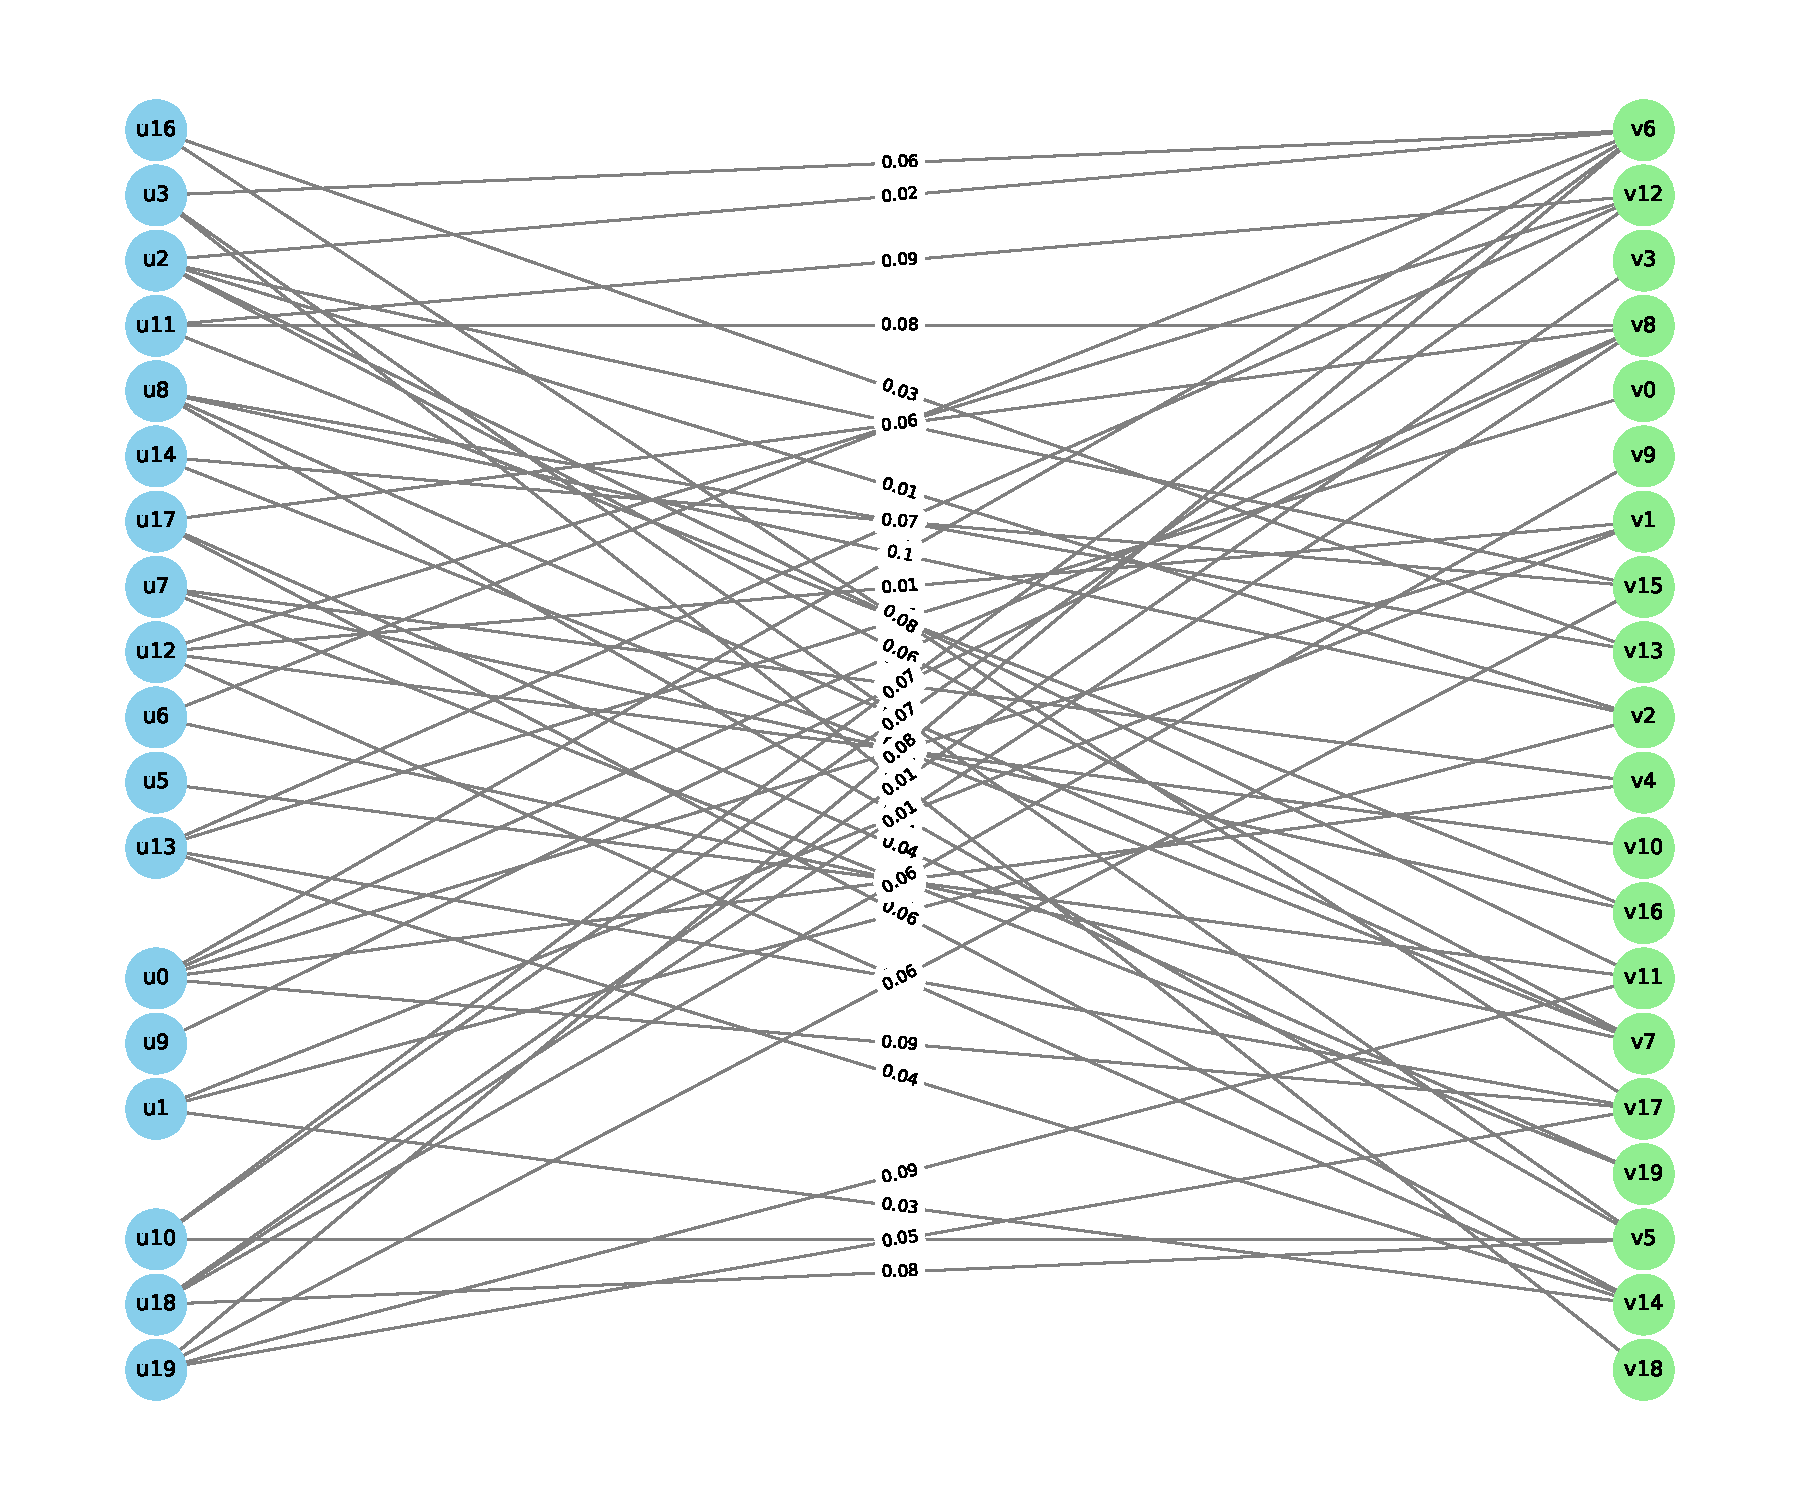
\includegraphics[width=1\linewidth]{img/graph_example.pdf}
    \caption{Bipartite Erdos Renyi random graph}
    \label{fig:erdos}
\end{figure}

\par
\hspace{\parindent}The advantage of this design is that we can deduce some properties and scores of an online algorithm with respect to the parameters of the graph generation ($p$, number of edges etc...). In our experiment, we evaluate an algorithm by its number of successful match. It is important to consider that in this setting, $OPT$ can be lower than the empirical result of an algorithm (since the empirical result is stochastic), in order to prevent it, we will run the algorithm $k$ time and take the empirical mean of the number of (successful) match. 

\subsection{Results}

\par
\hspace{\parindent}In order to evaluate the algorithms, we generate different graphs (representing different scenarios) and for each instance (ie graph) we evaluate the three algorithm présented: $NonAdaptive$, $StochasticBalance$ \& $SemiAdaptive$. The algorithm $Naive$ denotes the naive algorithm that chooses the available vertex $u$ with the highest probability. The version $NaiveAdap$ has the information if a vertex $u$ has already succeed or not and choose the vertex with the highest probability that is available. Our results presents the average score (over $k=20$ iterations) of the graphs when we modify the following parameters:

\begin{itemize}
    \item $U_n$ which denotes the number of vertex in $U$ (and $V$).
    \item $p_{erd}$ which denote the probability of two vertices $v_i$ and $u_i$ to be connected. We consider the cases where $p_{erd} = \frac{log(U_n)}{U_n}$ \& $p_{erd} = \frac{1}{U_n}$, we call them $highly$ and $sparse$ cases.
    \item $p_{uv}$ the probability of success for two vertices, it is either picked at random (uniformaly between 0 and $p_{max}$, or is equal to $p$ for all $u, v$.

\end{itemize}

\par
\hspace{\parindent}For every algorithm, we device its score by the score of $OPT$ on the graph for the corresponding \textit{Budget Allocation problem}. The results are presented in appendix.

\par
\hspace{\parindent}Here we can clearly see some interesting results. First, the performance of the algorithm (all of them) highly depends on the range of $p_{uv}$, we can see that for large values of $p$, the algorithm tends to have bad performances (compared to $OPT$) while when $p \approx 0$, the algorithms tends to show great performances. Furthermore, we can see that $NonAdaptive$ and $Naive$ shows a large contrast in their performances, while we do not observe a clear domination of $StochasticBalance$ and $NaiveAdapt$ when the all the $p_{uv}$'s are  equal. In fact, the $StochasticBalance$ was designed to manage the problem in the worst cases, so its advantages do not reveal clearly in random scenarios like the ones we generated.
\par
\hspace{\parindent}$SemiAdaptive$ algorithm shows good results too, however they are not way higher than $NaiveAdaptive$ or $StochasticBalance$ even in the case where then $p_{uv}$ are not restricted to an unique value. Actually, this algorithm was designed specifically to find a theoritical competitive ratio. We can see that the choice of doing "the best in the worst case" may not lead to impressive results on classical instances.

\section{Conclusion \& Discussion}

\par
\hspace{\parindent}Optimal Matching with Stochastic Rewards is a challenging problem. According to \cite{survey2024}, it remains an important open problem to design better online algorithms for less restriction on the probability range of the reward (sometimes called the \textit{Click Target Rate} (CTR), for its application on online advertisement). The presented algorithm holds for a small CTR but as we saw in the experimental part, the results do not hold when the CTR gets higher. Recent improvement in the online Primal Dual framework led to an improvement of the analysis of famous algorithm (such as $Ranking$ or $StochasticBalance$) and a better understanding of the problem under stochasticity (\cite{huang2023}). Future work focus on developing more robust algorithms that perform well across a broader range of CTRs, leveraging adaptive and hybrid approaches to address the problem's inherent complexities, and developing the theoretical framework to analyze the bounds of the problem under more realistic scenarios.


\clearpage
\onecolumn

\clearpage

\printbibliography
\clearpage
\null
\vfill
\begin{center}
\huge\textbf{Appendix}
\end{center}
\vfill
\thispagestyle{empty}
\newpage

\appendix

\section{Theorem 2: Proof}

We recall the proof of Theorem \ref{Theorem ranking} (same as the one given in class).

\begin{proof}
    For the optimal matching (that matches everyone), we denote $\Pi$ the chosen permutation. We say that $(\Pi, u)$ is a miss event at rank $t$ if $\Pi(u) = t$ and $u$ is not matched. Conversely, $(\Pi, u)$ is a match event if $u$ is matched.
    
    Our goal is to minimize the number of miss events. If $(\Pi, u^*)$ is a miss event, it means there exists $v^*$ which is matched with $u^*$ by OPT. Since $v^*$ is matched with some $u'$ (arbitrary), it follows that for each miss event, there exists a match event. Otherwise, $v^*$ and $u^*$ would both remain free and should be matched in the end. Thus, we obtain:
    \begin{align*}
        \#\{\text{miss events}\} + &\#\{\text{match events}\} = n, \\
        n \leq 2 \times &\#\{\text{match events}\}.
    \end{align*}
    This proves that $CR(\text{ranking}) \geq \frac{1}{2}$.
    
    Now, we aim to associate one miss event $(\Pi, u^*)$ with multiple match events for different permutations. We start with a ranking where $u^*$ is not matched. For this ranking, we define $\Pi^{(i)}$ as the permutation where $\Pi^{(i)}(u^*) = i$ and for all other $u > u'$, we have $\Pi^{(i)}(u) > \Pi^{(i)}(u')$ (preserving the relative order). To proceed, we introduce the following property:
    
    \begin{property}
        If $(\Pi, u)$ is a miss event and $\Pi(u) = t$, then there are $n$ match events $(\Pi^{(i)}, u)$ at position $s \leq t$.
    \end{property}
    
    The main idea here is that if $u^*$ is not matched because $v^*$ is matched with $u'$, then for all permutations such that $\Pi^{(i)}(u^*) \geq \Pi^{(i)}(u')$, $v^*$ will still match with $u'$. To be precise, this argument is not entirely rigorous because $v^*$ could also match with some $u''$, but it does not matter since $v^*$ never matches with $u^*$ in the optimal matching. By induction, we can conclude the property.
    
    Using this property, we observe that:
    \[
        n(1 - P_t) \leq \sum_{s=1}^{t} P_s,
    \]
    where $P_s$ is the probability of a match event at position $s$.
    
    The performance of the ranking algorithm is given by:
    \[
        \mathbb{E}[\text{number of match events}] = \sum_{s=1}^{t} P_s \geq \min_{P_1, P_2, \dots, P_n} \sum_{i=1}^{t} P_i,
    \]
    subject to the constraint:
    \[
        \forall t, \quad n(1 - P_t) \leq \sum_{s=1}^{t} P_s.
    \]
    
    Finally, we find that:
    \[
        P_i \geq \left( \frac{n}{n+1} \right)^i,
    \]
    and we conclude that:
    \[
        CR(\text{ranking}) = 1 - \frac{1}{e} + o(1).
    \]
\end{proof}


\section{Some details about the implementation}
For the implementation of $NonAdaptive$, in the pseudo code we use a table $w_i(u)$ of size $|V|\times |U|$. However we can see that we can simply use a table of size $u$ since at each iteration $t$, we only use the information of $w_{t-1}$, reducing the memory from $O(|V|\times |U)$ to $O(|U|)$.

In the algorithm $StochasticBalance$, we need to select the vertex $u$ with the least loads $L_u$. However many $u_i$ can be candidate so we select the one with the highest probability $p_{uv}$.

For the $Naive$ algorithm, we select the vertex $u$ with the highest probability $p_{uv}$. When $p_{uv}=p$, we select the first vertex $u$ available.

For the $SemiAdaptive$ algorithm, if a vertex $v$ has only one possible match $u$, we simply match them and update $FirstSucc(1)$ only if it was a success.

\newpage
\section{Results}

\begin{table}[h]
    \centering
    \renewcommand{\arraystretch}{1.}
    \setlength{\tabcolsep}{6pt}
    \begin{adjustbox}{max width=\textwidth}
    \begin{tabular}{cccccccc}
        \toprule
        \multirow{2}{*}{\textbf{$p_{uv}$}} & \multirow{2}{*}{\textbf{$U_n$}} & \multirow{2}{*}{\textbf{$p_erd$}} & \multicolumn{5}{c}{\textbf{Algorithm}} \\
        \cmidrule(lr){4-8}
        & & & Naive & NonAdaptive & NaiveAdaptive & StochasticBalance & SemiAdaptative \\
        \midrule
        \multirow{9}{*}{random} & \multirow{3}{*}{20} & 0.2 & 0.26 & 0.53 & 0.56 & 0.38 & 0.44 \\
        & & sparse & 0.39 & 0.44 & 0.56 & 0.33 & 0.50 \\
        & & highly & 0.26 & 0.41 & 0.52 & 0.44 & 0.48 \\
        \cmidrule(lr){2-8}
        & \multirow{3}{*}{50} & 0.2 & 0.31 & 0.46 & 0.56 & 0.51 & 0.42 \\
        & & sparse & 0.48 & 0.50 & 0.50 & 0.37 & 0.37 \\
        & & highly & 0.37 & 0.52 & 0.59 & 0.48 & 0.45 \\
        \cmidrule(lr){2-8}
        & \multirow{3}{*}{150} & 0.2 & 0.27 & 0.44 & 0.51 & 0.49 & 0.43 \\
        & & sparse & 0.44 & 0.55 & 0.52 & 0.64 & 0.48 \\
        & & highly & 0.34 & 0.46 & 0.52 & 0.48 & 0.46 \\
        \midrule
        \multirow{9}{*}{0.5} & \multirow{3}{*}{20} & 0.2 & 0.04 & 0.10 & 0.10 & 0.10 & 0.10 \\
        & & sparse & 0.09 & 0.09 & 0.09 & 0.09 & 0.09 \\
        & & highly & 0.05 & 0.10 & 0.10 & 0.10 & 0.10 \\
        \cmidrule(lr){2-8}
        & \multirow{3}{*}{50} & 0.2 & 0.02 & 0.10 & 0.10 & 0.10 & 0.10 \\
        & & sparse & 0.08 & 0.13 & 0.13 & 0.13 & 0.13 \\
        & & highly & 0.05 & 0.10 & 0.10 & 0.10 & 0.10 \\
        \cmidrule(lr){2-8}
        & \multirow{3}{*}{150} & 0.2 & 0.01 & 0.10 & 0.10 & 0.10 & 0.10 \\
        & & sparse & 0.08 & 0.11 & 0.11 & 0.11 & 0.11 \\
        & & highly & 0.04 & 0.10 & 0.10 & 0.10 & 0.10 \\
        \midrule
        \multirow{9}{*}{0.1} & \multirow{3}{*}{20} & 0.2 & 0.20 & 0.38 & 0.50 & 0.50 & 0.48 \\
        & & sparse & 0.29 & 0.33 & 0.38 & 0.38 & 0.38 \\
        & & highly & 0.28 & 0.44 & 0.50 & 0.53 & 0.42 \\
        \cmidrule(lr){2-8}
        & \multirow{3}{*}{50} & 0.2 & 0.12 & 0.43 & 0.50 & 0.50 & 0.44 \\
        & & sparse & 0.35 & 0.40 & 0.44 & 0.37 & 0.39 \\
        & & highly & 0.22 & 0.43 & 0.50 & 0.49 & 0.38 \\
        \midrule
        \multirow{9}{*}{0.05} & \multirow{3}{*}{20} & 0.2 & 0.40 & 0.65 & 0.75 & 0.75 & 0.65 \\
        & & sparse & 0.33 & 0.67 & 0.73 & 0.67 & 0.53 \\
        & & highly & 0.41 & 0.76 & 0.88 & 0.88 & 0.88 \\
        \cmidrule(lr){2-8}
        & \multirow{3}{*}{50} & 0.2 & 0.18 & 0.64 & 0.68 & 0.72 & 0.74 \\
        & & sparse & 0.43 & 0.49 & 0.49 & 0.69 & 0.71 \\
        & & highly & 0.33 & 0.65 & 0.69 & 0.86 & 0.63 \\
        \cmidrule(lr){2-8}
        & \multirow{3}{*}{150} & 0.2 & 0.09 & 0.64 & 0.60 & 0.71 & 0.62 \\
        & & sparse & 0.55 & 0.57 & 0.61 & 0.69 & 0.61 \\
        & & highly & 0.30 & 0.60 & 0.82 & 0.83 & 0.62 \\
        \bottomrule
    \end{tabular}
    \end{adjustbox}
    \caption{Results on Erdos Renyi generated graphs.}
    \label{tab:results}
\end{table}

\end{document}


\clearpage
\onecolumn
\printbibliography
\end{document}
